\section{Лекция 25 (17.05.25)}

\subsection{Параллельные методы решения задач гидродинамики}
\clisting{open}{"../doc/parallel_examples.cpp"}
\subsubsection{Распараллеливание циклов и явных схем}
Рассмотрим явную схему против потока для одномерного уравнения переноса:
\clisting{block}{"void explicit_step("}
Параллельная версия этого цикла с использованием библиотеки {\bf OpenMP} будет иметь вид
\clisting{block}{"void explicit_step("}

Та же схема с использованием системных потоков \cvar{std::thread}:
\clisting{block}{"void explicit_step("}

\subsubsection{Параллельное решение независимых подзадач}
Псевдокод решения  нескольких дифференциальных уравнений
для трёхмерного segragated метода: уравнения для компонент скорости
могут быть решены независимо друг от друга в разных потоках.
Используем для их решения асинхронное программирование
\clisting{lines-range}{"std::vector", ";//"}


\subsubsection{Domain Decomposition Method. Метод Шварца}

\begin{figure}[h!]
\centering
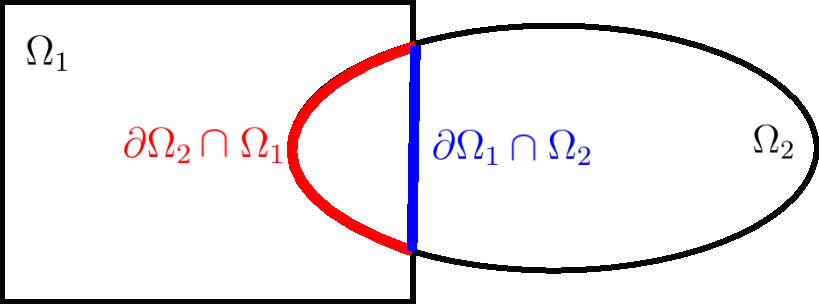
\includegraphics[width=0.4\linewidth]{schwarz_domain.pdf}
\caption{Область решения $\Omega$, разбитая на два перекрывающихся поддомена $\Omega_1$, $\Omega_2$}
\label{fig:scwarz_domain}
\end{figure}

Постановка задачи на итерации Шварца $n+1$ для $i$-го домена имеет вид
\begin{equation}
\begin{cases}
\label{eq:schwarz_iprob}
-\nabla^2 u_i^{n+1} = f, \qquad &x\in\Omega_i,  \\
u_i^{n+1} = b, \qquad &x\in\partial\Omega \cap \partial\Omega_i, \\
u_i^{n+1} = u^n, \qquad &x\in\partial\Omega_i \cap \Omega_j.
\end{cases}
\end{equation}
где функция глобального решения на итерации определяется как
\begin{equation}
\label{eq:schwarz_un}
u^n = \sum_i E_i\left(\Chi_i \, u_i^{n}\right).
\end{equation}
Здесь $E_i$ -- функционал, расширяющий функцию, заданную в домене $\Omega_i$ на область $\Omega$, дополняя эту функцию нулями.
$\Chi_i$ -- ограничивающий весовой коэффициент, обеспечивающий корректное поведение глобальной функции в зонах перекрытия.
\begin{equation}
\label{eq:schwarz_chi}
\begin{aligned}
& \Chi_i = \begin{cases}
   1, \qquad &\Omega_i \backslash \cup \Omega_j, \\
   0, \qquad &\cup \Omega_j \backslash \Omega_i, \\
   [0, 1], \quad & \Omega_i \cap \Omega_j
  \end{cases} \\
& \sum_i \Chi_i = 1.
\end{aligned}
\end{equation}

В зависимости от того, когда происходит вычисление глобальной функции, алгоритм Шварца можно
использовать как в последовательном, так и в параллельном виде.
Так, если обновлять глобальное решение $u^n$ \cref{eq:schwarz_un} после решения
для каждого поддомена $\Omega_i$ \cref{eq:schwarz_iprob}, то получим последовательный (классический) алгоитм Шварца.
Если же обновлять глобальное решение один раз на итерации после расчёта всех поддоменов, то
получим параллельный алгоритм.
Можно провести аналогию с итерационными алгоритмами решения систем линейных уравнений:\
последовательный алгоритм соответствуюет методу Зейделя, а параллельный -- методу Якоби. 

\subsubsubsection{Построение сетки для конечнообъёмного DDM-метода}
\label{sec:schwarz_fem_grid}

\begin{figure}[h!]
\centering
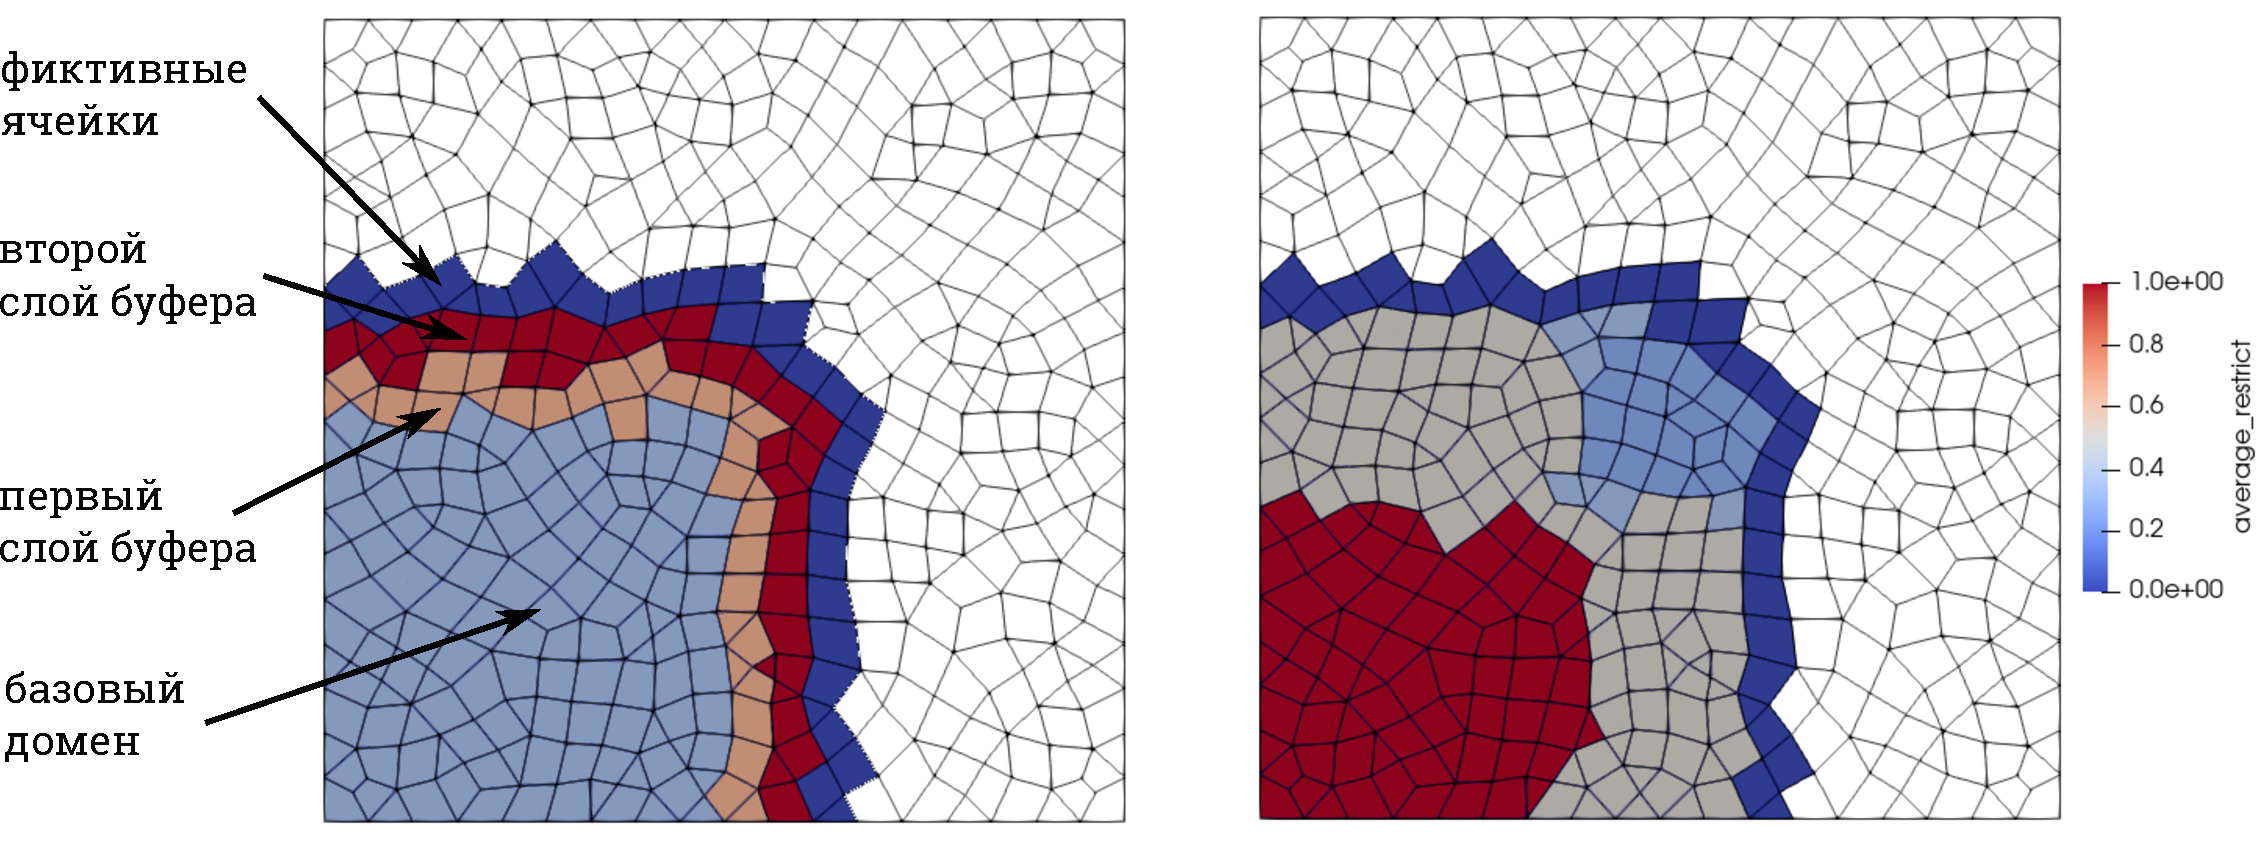
\includegraphics[width=0.9\linewidth]{schwarz_grid.pdf}
\caption{Сетка в левом нижний домене при разбиении квадрата по схеме $2\times2$. Слева -- буферные слои, справа -- усреднённая весовая функция $\Chi$}
\label{fig:schwarz_grid}
\end{figure}

\begin{enumerate}
\item На первом этапе вся расчётная область покрывается единой конечнообъёной сеткой.
\item Для каждого домена определяется набор ячеек из общей сетки, принадлежащих этому домену. На рис.~\ref{fig:schwarz_grid}
эта зона обозначена как <<базовый домен>>. Таким образом строится набор неперекрывающихся сеток.
\item Строится буферная зона (зона перекрытия). От каждой базовой сетки отмечается ряд внешних соседних ячеек. Так делается несколько раз в зависимости от количества буферных слоёв.
      На рис.~\ref{fig:schwarz_grid} отмечены два буферных слоя.
\item По такому же принципу отмечается ещё один слой фиктивных ячеек (ghost cells). Эти ячейки будут использоваться для постановки условия
      на междоменной границе (последнее из условий \cref{eq:schwarz_iprob}).
\item Для каждого домена строится весовая функция $\Chi$, удовлетворяющая условию \cref{eq:schwarz_chi}.
      В простейшем случае можно использовать среднее арифметическое: $\Chi_i = 1/N_d$ - где $N_d$ -- количество доменов, содерижащих текущую точку области.
      На рис.~\ref{fig:schwarz_grid} справа представлена такая функция. В зависимости от ячейки её значения варьируются между $1, 1/2, 1/3, 1/4, 0$.
      Отметим, что в слое фиктивных ячеек весовая функция равна нулю, так как этот формальный слой используется только для удобного задания условий Дирихле
      при сборке СЛАУ методом конечных объёмов.
\end{enumerate}

\subsubsubsection{MPI реализация конечнообъёмного метода Шварца}
Ниже представлена MPI реализаиция метода Шварца в параллельной постановке
\clisting{block}{"int main"}


\subsubsection{Задание для самостоятельной работы}
В файле \ename{"poisson_fvm_solve_test.cpp"}
реализован тест \cvar{"[poisson2-fvm-ddm"]"},
в котором решено уравнение Пуассона в единичном квадрате на неструктурированной сетке.
Используется метод Шварца в последовательной постановке.

В программе после чтения сетки тестовая задача сначала решается на одном домене. Для
сравнения с результатами DDM-метода.
Файл с сеткой ищется либо в директории, в которой находится программа, либо в корневой для репозитория папке \ename{test_data}.

Далее строятся поддомены на основе регулярного разбиения квадрата на основе алгоритма, описанного в \ref{sec:schwarz_fem_grid}.
В строке
\clisting{open}{"test/poisson_fvm_solve_test.cpp"}
\clisting{line}{"GridPartition gridpart = "}
задаётся разбиение области.
Аргументы этого вызова соответствуют
\begin{itemize}
\item \cvar{grid} -- исходная сетка,
\item \cvar{{1, 2}} -- регулярное разбиение домена. В данном случае по оси x используется один участок, по оси y -- два.
То есть построено два поддомена примерно соответсвующих областям $y\in[0, 0.5]$  и $y\in[0.5, 1.0]$.
\item \cvar{2} -- количество буферных слоёв ячеек. Для первого домена буферная зона начинается за $y>0.5$.
\item \cvar{1} -- количество слоёв с фиктивными ячейками (ghost cells).
\end{itemize}

Далее строится средняя арифметическая весовая функция для каждого поддомена \cvar{Xi} 
и строится аппроксимация задач \cref{eq:schwarz_iprob} в каждом домене.
Итогом сборки являются матрицы \cvar{local_mat}, правые части \cvar{local_rhs}
и решатели СЛАУ \cvar{local_solver}.

Далее происходит инициализация сохранения итерационного решения в vtk \cvar{writer}.
Программа печатает в консоль невязку после каждой из итераций и создаёт файл \ename{schwarz_ddm_poisson.vtk.series}
для Paraview, в котором можно посмотреть как само решение на итерационном слое (поле solution) так и отличие от решения, полученного на едином домене (поле error).

Потом начинаются итерации Шварца.
Для каждого домена обновляются граничные условия на местах состыковки доменов (условия в фиктивных ячейках -- аналог последнего из условий \cref{eq:schwarz_iprob})
и решается СЛАУ.
Поскольку представлена последовательная реализация алгоритма, то после каждого решения в домена
происходит обновление глобального решения по формуле \cref{eq:schwarz_un}.

Завершают итеарцию вывод информации и сохранением решения.

\subsubsubsection{Необходимо}

\begin{enumerate}
\item Проиллюстрировать сходимость последовательного метода Шварца с помощью визуализации решения и ошибки. Использовать подробную сетку (например, tetragrid с 10 тысяч ячеек).
      Использовать разбиение по доменам $3\times3$.
\item Изменить программу для реализации параллельного метода Шварца. Аналогично проиллюстрировать его работу.
\item Построить сравнительные графики уменьшения невязки с продвижением по итерациям для разных величин буферных зоны. Использовать последовательный и параллельный методы.
\item Реализовать параллельную версию алгоритма Шварца на MPI. Замерить время работы отдельных составных частей внутри итерационного цикла: построение правой части, вычисление невязки, решение локальной СЛАУ, обновление глобального решения. Вывести результаты для нескольких разбиений: например $1\times2$, $2\times2$, $4\times4$, $8\times8$. Интересует как общее время по всем итерациям, так и время, нормированное на одну итерацию (то есть общее время, делённое на количество итераций).
\item Запустить MPI программу на двух компьютерах, находящихся в одной локальной сети. Посчитать время аналогично предыдущему пункту.
\end{enumerate}

\subsubsubsection{Рекомендации к программированию}
Для изменения алгоритма с последовательного на параллельный достаточно вынести блок , отвечающий за обновление глобального решения (\cvar{//update global solution}),
из цикла по доменам (\cvar{idom}).

Тестовая MPI программа (слинкованная с библиотекой \ename{cfd24}) лежит в папке \ename{src/mpi_test}.
Чтобы активировать её сборку нужно запустить cmake с флагом (если из папки \ename{build})
\begin{bashcode}
cmake .. -DCMAKE_BUILD_TYPE=Release -DMPI_TESTS=ON
\end{bashcode}
Для сборки MPI программы необходимо установить в систему реализацию MPI (например OpenMPI, MSMPI, MPICH и др.)

После этого процедура сборки будет вместе с иходной программой \ename{cfd24_test} также будет собирать программу \ename{mpi_cfd24_test}.
В этой программе реализован простой тест (\cvar{simple_mpi_test}) на сложение чисел, лежащих в разных потоках с помощью редукции.
Если система настроена правильно, то эта программа должна запускаться и не давать ошибок. Например, запуск на 8 потоках (добавить exe для Windows)
\begin{bashcode}
mpirun -H localhost:8 mpi_cfd24_test 
\end{bashcode}

В этой же программе в файле \ename{ddm_poisson_test} есть функция \cvar{schwarz_ddm_poisson_test}
которая читает расчётную сетку. Программу расчёта нужно дописывать в эту функцию.
При переводе последовательной программы в параллельную необходимо
избавиться от всех циклов по доменам (\cvar{idom}). Теперь индексу домена будет соответствовать индекс ранга (\cvar{mpi_rank}).
Также все переменные, заданные в домене (именованные по шаблону \cvar{local_*})
должны перестать быть векторами. Например, \cvar{local_mat} в оригинальной программе -- это массив из матриц (\cvar{vector<CsrMatrix>}).
В MPI программе это будет просто матрица (\cvar{CsrMatrix}) для текущего ранга.
Полную проблему (\cvar{full_worker}) в MPI версии делать не обязательно.
Соответственно и сравнения с полной и DDM результатов тоже не нужно (расчёт поля \ename{error}).

Замер времени расчёта нужно проводить только в одном ранге (нулевом).

Количество потоков, с которыми запускается программа должна соответсвовать количеству доменов.
Например, если вы используете разбиение по дооменам $2\times2$, то программу нужно запускать на 4-х потоках.

Для запуска программы на нескольких компьютерах нужно
\begin{enumerate}
\item Подключить два компьютера с одинаковой операционной системой к одной локальной сети. Например, к одной сети WiFi
\item Узнать локальные адреса этих компьютеров в этой сети
\item Обеспечить ssh доступ с основного комьютера на все остальные без пароля (по ssh ключу) и с дефолтным пользователем.
      С основного компьютера ssh подключение должно создаваться по (вместо 192.168.1.2 подставить адрес второго компьютера)
\begin{bashcode}
ssh 192.168.1.2
\end{bashcode}

\item Положить скомпилированную программу \cvar{mpi_cfd24_test} в одно и тоже место на этих компьютерах. Рядом положить целевую сетку
\item Для запуска на 4-х потоках (по два на компьютер) нужно на основном компьютере запустить (заменить \ename{192.168.1.2} на адрес второго компьютера, \ename{/home/user/...} на полный путь к программе).
\begin{bashcode}
mpirun -H localhost:2,192.168.1.2:2 /home/user/mpitest/mpi_cfd24_test
\end{bashcode}
\end{enumerate}
